\section{Data samples}
\label{sec:kstmm:data}

This section describes the data and simulation samples used in the angular analysis of \BdToKstmm.
The second set of data is a superset of the first but processed with a later version of the reconstruction and event selection software.
There are two distinct versions of simulated events, one representing the data-taking conditions
and detector knowledge at the end of 2010 (MC10) and the second representing the equivalent conditions for the 2011 data-taking period (MC11).
The MC11 samples were only used in the second angular analysis.

\subsection{Data}

\subsubsection{Sample 1 - 0.38\invfb }

The  dataset used in the first analysis of \BdToKstmm at \lhcb was collected between March and June 2011.
The data was taken at a centre-of-mass energy of $\sqs=7\tev$ using both polarities of the \lhcb magnet.
The data sample corresponds to an integrated luminosity of 0.38\invpb.
The vast majority of data was taken in the trigger configuration using the multi-variate topological trigger % labelled \verb=0x006d0032=,
 with smaller samples being taken in almost identical conditions throughout the year.
The data are reconstructed with reconstruction version \verb=Reco10=, as described in Section~\ref{sec:lhcb:soft},
 and stripped with version \verb=Stripping13b=, described in detail below.

\subsubsection{Sample 2 - 1.0\invfb }

The dataset used in the second angular analysis of \BdToKstmm at \lhcb was the full dataset from the 2011 run of the \lhc.
This corresponds to an integrated luminosity of 1.0\invfb of data at a centre-of-mass energy of $\sqs=7\tev$.
The trigger configuration was consistent throughout 2011 for the trigger lines used to select events in the angular analysis.
The reconstruction and the event selection are consistent for the whole dataset.
The particular versions of the reconstruction and event selection software used are \verb=Reco12= and \verb=Stripping17= respectively.


\subsection{Simulation}
\label{sec:kstmm:data:mc}

The samples of simulation used in the angular analysis were generated as outlined in Sec.~\ref{sec:lhcb:soft}.
The generation and reconstruction conditions of each sample are described in detail below.
To ensure that the correct efficiency is calculated from the simulation, the properties 
of the simulation are compared with large data control samples.
In order to update the simulations to agree with the best knowledge of the detector in 2011,
the set of corrections derived in Section~\ref{sec:kstmm:data:mccorr} was checked using \BdToJpsiKstar data and simulation.

\subsubsection{MC10}


The samples of MC10 that were used for both angular analyses were 
simulated to be a close approximation of the data-taking conditions 
in 2010. % by using the latest versions of the trigger, reconstruction, and stripping software.
In order to use this simulation with the 2011 data, an updated version of the trigger and
event selection software was re-run over the simulated events.
The sample of simulated events generated in the MC10 configuration was of \BdToKstmm events.
This sample was generated using a decay model such that the events are flat in phase space and therefore 
have a uniform distribution in \ctl, \ctk and $\phi$. 
The distribution of phase space events in \qsq decreases as 
the size of the phase space available for the decay at higher \qsq values gets smaller.
The generator level distribution for \qsq is shown in Fig.~\ref{fig:phspqsq}.
\begin{figure}[tbp]
\centering
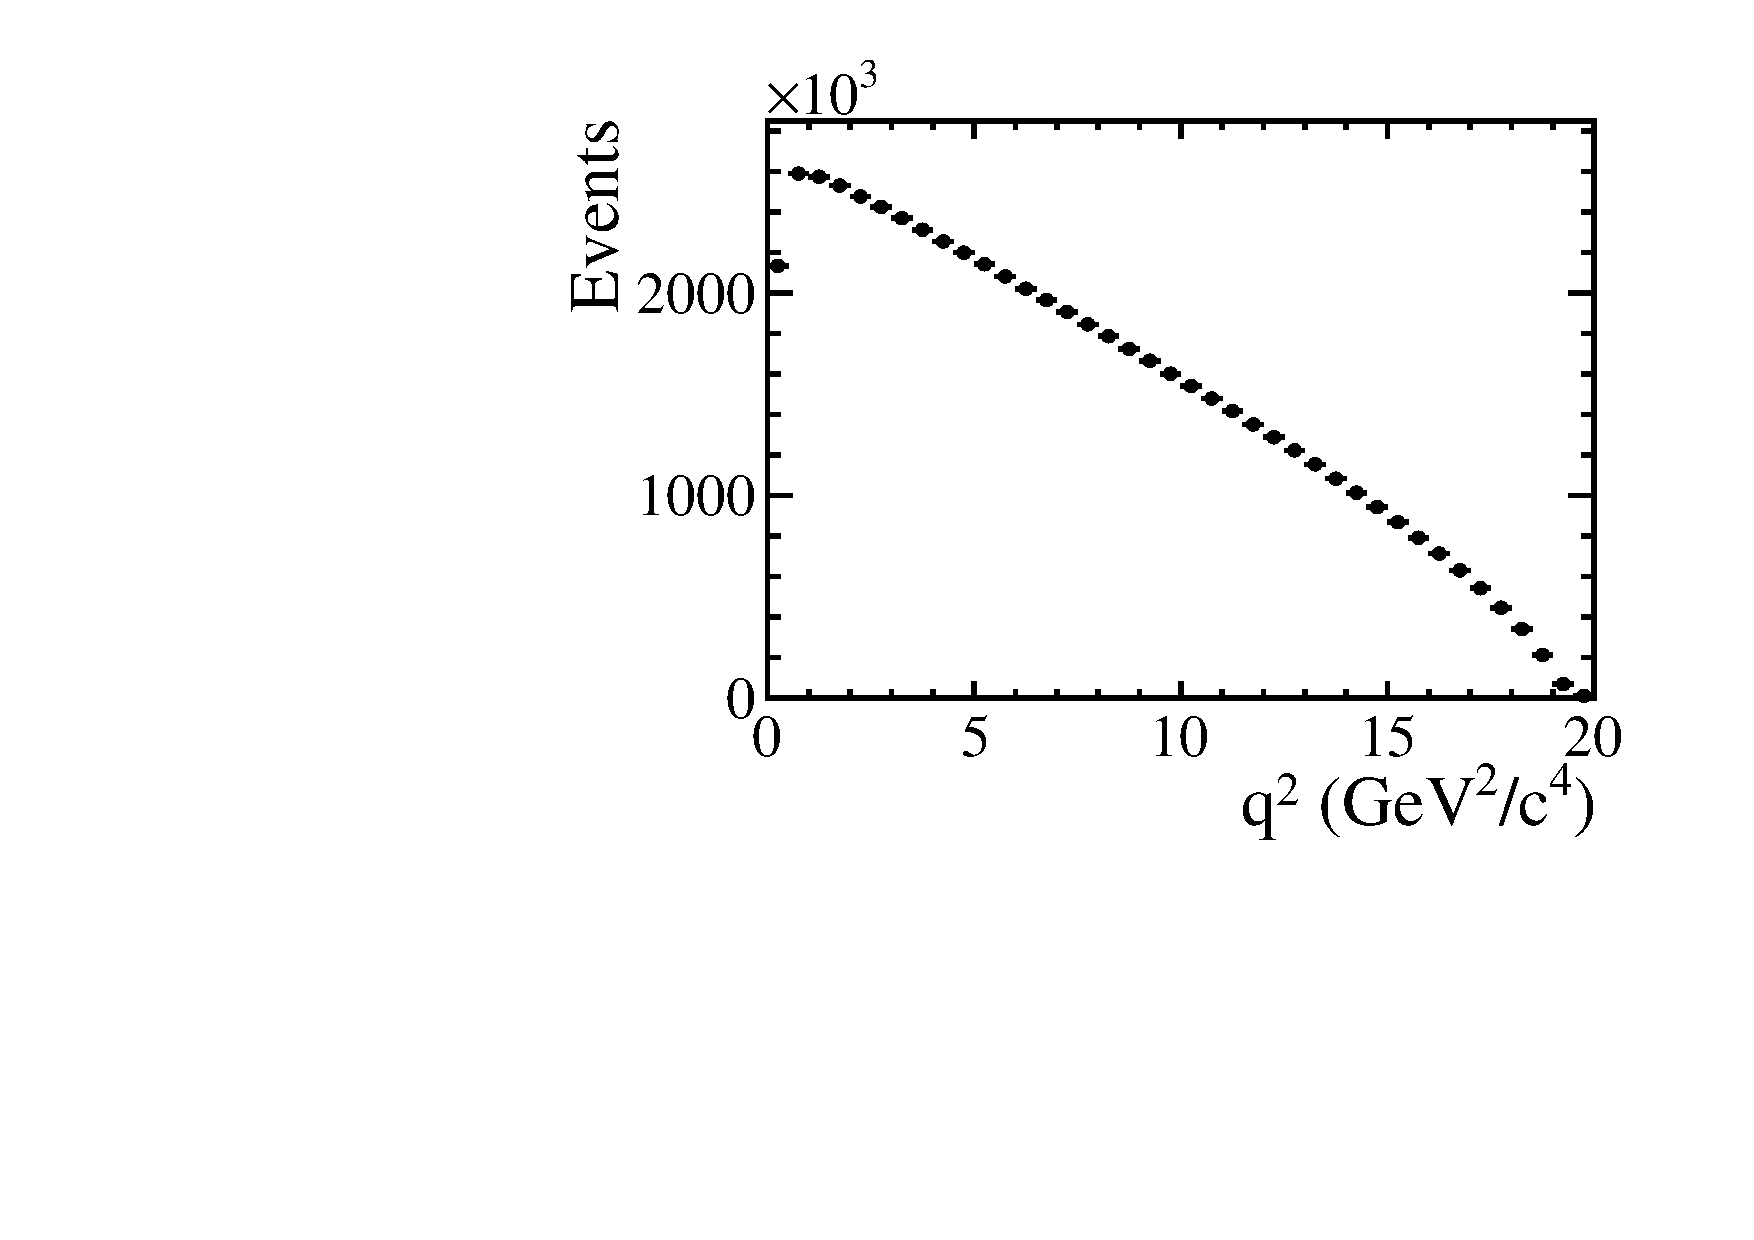
\includegraphics[width=0.48\columnwidth]{chapter5/figs/phsp_qsq_dist.pdf}
\caption[  The \qsq distribution of simulated \BdToKstmm events.  ]
{ The \qsq distribution of simulated \BdToKstmm events 
generated using a phase space model. The phase space available 
for the decay decreases towards high \qsq. The distribution of events is uniform in \ctl, \ctk and $\phi$.
 ~\label{fig:phspqsq} } 
\end{figure}
This sample of simulated events was used to calculate the efficiency to correct for the acceptance effects, as described in Sec.~\ref{sec:kstmm:ac}.

\subsubsection{MC11}

The samples of MC11 that were used in the second angular analysis of \BdToKstmm
consist of several signal decay modes, including \BdToKstmm, \BdToJpsiKstar, \BuToKmm, \BuToKstmm, \BsToPhimm and \LbToLmm.
The \B decays  were generated using the \verb=BTOSLLBALL=~\cite{PhysRevD.61.074024} model from \evtgen~\cite{Lange:2001uf}
to model the \bquark\to\squark FCNC decay.
This model calculates the helicity amplitudes for the \Bd\to\Kstarz transition using the form factors
calculated with the QCD sum rule using Standard Model parameters.
For the generation of the non-\Bd modes decays, the same model is used based on the assumption
 that the masses and kinematic distributions of the parent and daughter particles are approximately equal.
The \Lb decay was generated uniformly in phase space.
The \BdToJpsiKstar simulation was also used to test the corrections applied to the phase space \BdToKstmm sample
 to make the data match the simulation and determine the accuracy of any corrections applied.
All of the samples were used to determine the level of irreducible `peaking' background decays 
that satisfy all the selection criteria and may introduce a systematic bias. 

\subsubsection{Data-simulation validation}

The complete set of data-simulation corrections described previously were verified by applying the procedure to simulated \BdToJpsiKstar candidates. 
The distribution of the BDT response of the \BdToJpsiKstar candidates in data and simulation is given in Fig~\ref{fig:bdtcomparison}.
\begin{figure}[tbp]
\centering
\subfigure[BDT distribution]{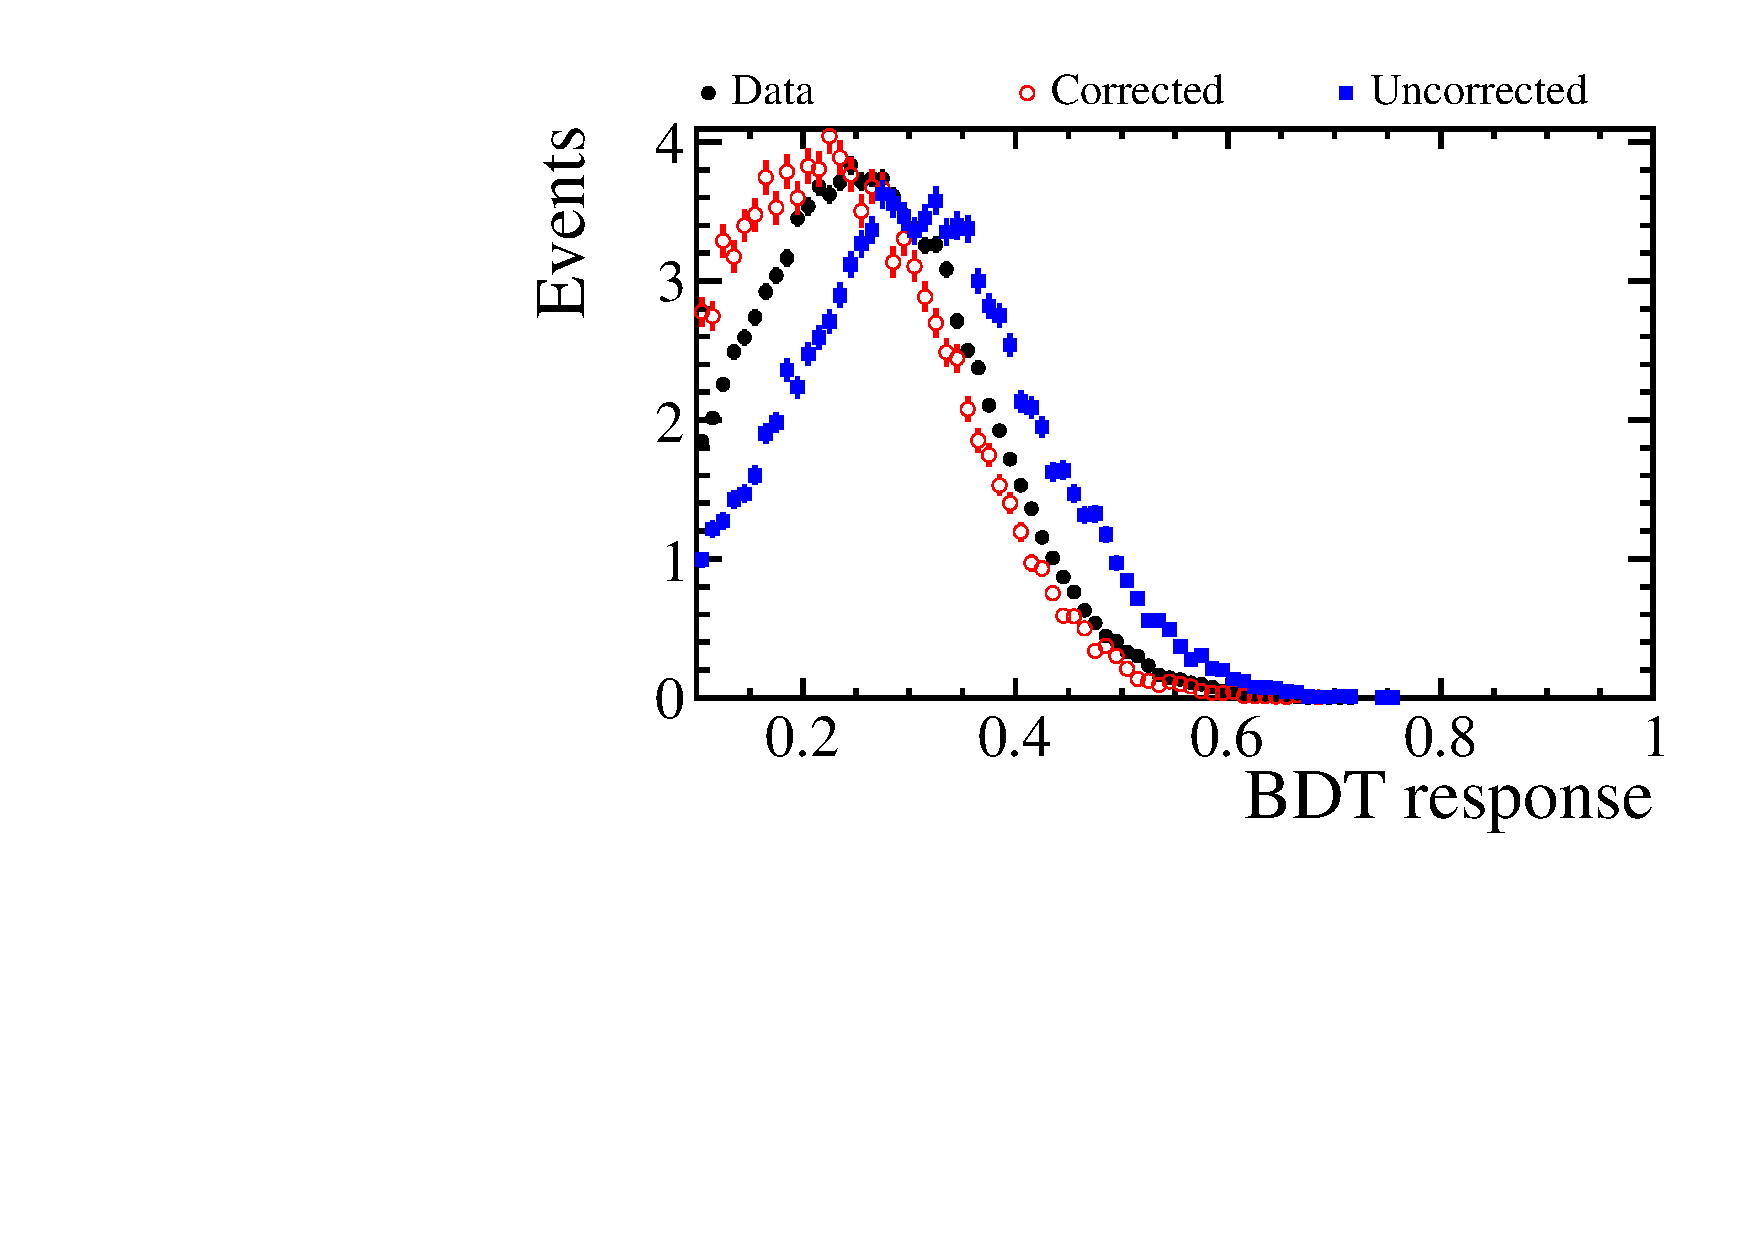
\includegraphics[width=0.48\columnwidth]{appendix/figs/comp_jpsikstar_default_BDT.pdf}}
\caption[The distribution of MVA classification values for \Bd\to\jpsi\Kstarz candidates from data and simulation.    ]
{The distribution of MVA classification values for \Bd\to\jpsi\Kstarz candidates from data and simulation.
The MVA is described in Sec~\ref{sec:kstmm:sel}. The data (black) is from the 1.0\invfb sample. 
The corrected (\textcolor{red}{red}) and uncorrected (\textcolor{blue}{blue}) 
 \BdToJpsiKstar candidates are from the same MC11 simulation sample.
~\label{fig:bdtcomparison}}
\end{figure}
There is good agreement between the data and the corrected-simulated candidates, 
giving confidence that the set of corrections replicates the BDT selection efficiency correctly.



